\section{The Project}
\sectiontoc

\subsection{Goals and Priorities}

\begin{frame}{Goals}

    \makebox[\textwidth][c] {
        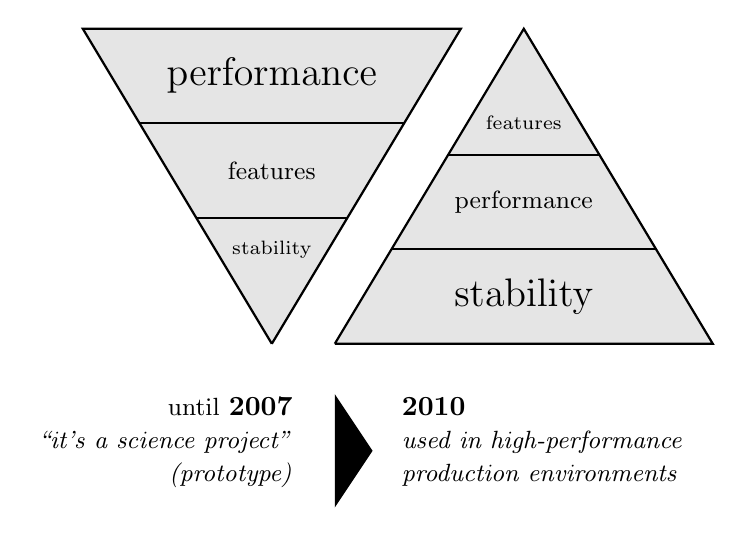
\begin{tikzpicture}[scale=0.8]
            \draw[thick,fill=black!10!white]
                (0, 0) -- (3, 5) -- (-3, 5) -- (0, 0);

            \draw[thick]
                (-2.1, 3.5) -- (2.1, 3.5)
                (-1.2, 2) -- (1.2, 2);

            \node (p1) at (0, 1.5) {\scriptsize stability};
            \node (p2) at (0, 2.75) {\small features};
            \node (p3) at (0, 4.25) {\Large performance};

            \node[align=right,anchor=north] (p7) at (-1.7, -0.7) {{\small{}until} \textbf{2007}\\
                \small\textit{``it's a science project''}\\
                \small\textit{(prototype)}};

            \draw[thick,fill=black!10!white]
                (1, 0) -- (4, 5) -- (7, 0) -- (1, 0);

            \draw[thick]
                (1.9, 1.5) -- (6.1, 1.5)
                (2.8, 3) -- (5.2, 3);

            \node (p6) at (4, 0.75) {\Large stability};
            \node (p5) at (4, 2.25) {\small performance};
            \node (p4) at (4, 3.5) {\scriptsize features};

            \node[align=left,anchor=north] (p8) at (4.3, -0.7) {\textbf{2010}\\
                \small\textit{used in high-performance}\\
                \small\textit{production environments}};

            \fill[fill=black]
                (1.0, -0.8) -- (1.6, -1.7) -- (1.0, -2.6);
        \end{tikzpicture}
    }

    \hfill\tiny reproduced from \cite{rock-hard}
\end{frame}

\subsection{History}
\begin{frame}{History}
    \begin{itemize}
        \item Started as a research project in 1999 by Peter Braam
        \item Braam founds \textbf{Cluster File Systems}
        \item Lustre 1.0 released in 2003
        \item \textbf{Sun Microsystems} aquires Cluster File Systems in 2007
        \item \textbf{Oracle Corporation} aquires Sun Mircrosystems in 2010
        \item Oracle ceases Lustre development, many new Organizations continue
            development, including \textbf{Xyratex},  \textbf{Whamcloud}, and
            more
        \item In 2012, \textbf{Intel} aquires Whamcloud
        \item In 2013, Xyratex purchases the original Lustre trademark from Oracle
    \end{itemize}
\end{frame}

\subsection{Who is involved?}
\begin{frame}{Who is involved?}
    \begin{description}
        \item[Oracle] \emph{no development}, only pre-1.8 support
        \item[Intel] funding, preparing for \emph{exascale computing}
        \item[Xyratex] hardware bundling
        \item[OpenSFS] (Open Scalable File Systems) ``keeping Lustre open''
        \item[EOFS] (EUROPEAN Open File Systems) (community collaboration)
        \item[FOSS Community] many joined one of the above to help development
            (e.g. Braam works for Xyratex now)
        \item[DDN, Dell, NetApp, Terascala, Xyratex]\hfill \\
            storage hardware bundled with Lustre
    \end{description}
\end{frame}

\begin{frame}{Supercomputers}
    \begin{quote}
        Lustre File System is managing data on more than 50 percent of the top
        50 supercomputers and seven of the top 10 supercomputers.

        \hspace*\fill{\scriptsize--- hpcwire.com, 2008 \cite{usage-stats}}
    \end{quote}

    \vspace{0.5cm}

    \begin{quote}
        The biggest computer today (\emph{Titan} by Cray, \#1 on TOP500) uses Lustre.
    \end{quote}

    \center\includegraphics[width=0.7\textwidth]{gfx/titan.jpg}\cite{titan-image}
\end{frame}
